\chapter{Evaluation} \label{chap:Evaluation}
%\begin{flushright}{\slshape    
%   Science, my boy, is made up of mistakes, but they are mistakes
%   which it is useful to make, because they lead little by little
%   to the truth}. \\ \medskip --- \citeauthor{verne_journey:1957}
%   \citetitle{verne_journey:1957} \citeyear{verne_journey:1957}
%\end{flushright} 

\lettrine[lines=4]{\textcolor{purple}{I}}{n} this chapter we describe the experiments we have performed to evaluate the feasibility and quality of the solution and to address the research questions identified in  \MySec{sec:solution_contribution}. The evaluation took place by using  \tool, which is the integration of \dSymb with \cSpark, to control the parallel execution of the Spark applications.

\section{Test Environment}\label{sec:test_env}
The test environment was built on Virtual Machines (from here onward VMs) of type   \textit{Standard\_D14\_v2}~\cite{AzureVMsizes}  provided by Microsoft Azure~\cite{AzureVM}, each of them equipped with $5$ CPUs, $112$ GiB of memory, $800$ GiB of local SSD memory and $6000$ Mbps of network bandwidth.
This type of VM is optimized for memory usage, with a high memory/core ratio. The os and software packages installed on these VMs are: Canonical Ubuntu Server 14.04.5-LTS~\cite{Ubuntu}, Oracle Java 8~\cite{Java8}, Apache Hadoop 2.7.2~\cite{Hadoop}, Apache Spark 2.0.2~\cite{Spark} and xSpark. All VM software is stored in a 200 GiB virtual hard drive maintained in the persistent layer of an Azure Blob Storage [24]. The VMs are organized in clusters composed of $5$ VMs running HDFS (storing the input datasets) and $5$ hosting Apache Spark and xSpark ($5$ for old \cSpark and $5$ for $\cSpark+\dSymb$). The Spark cluster runs Spark application either under Spark with the default configuration or under  $\cSpark+\dSymb$ or \cSpark with the configuration parameters shown in  \MyFig{fig:xSparkDagSymbConfigParms} or in \MyFig{fig:xSparkConfigParms} respectively.
\begin{figure}[thbp]
	\centering
	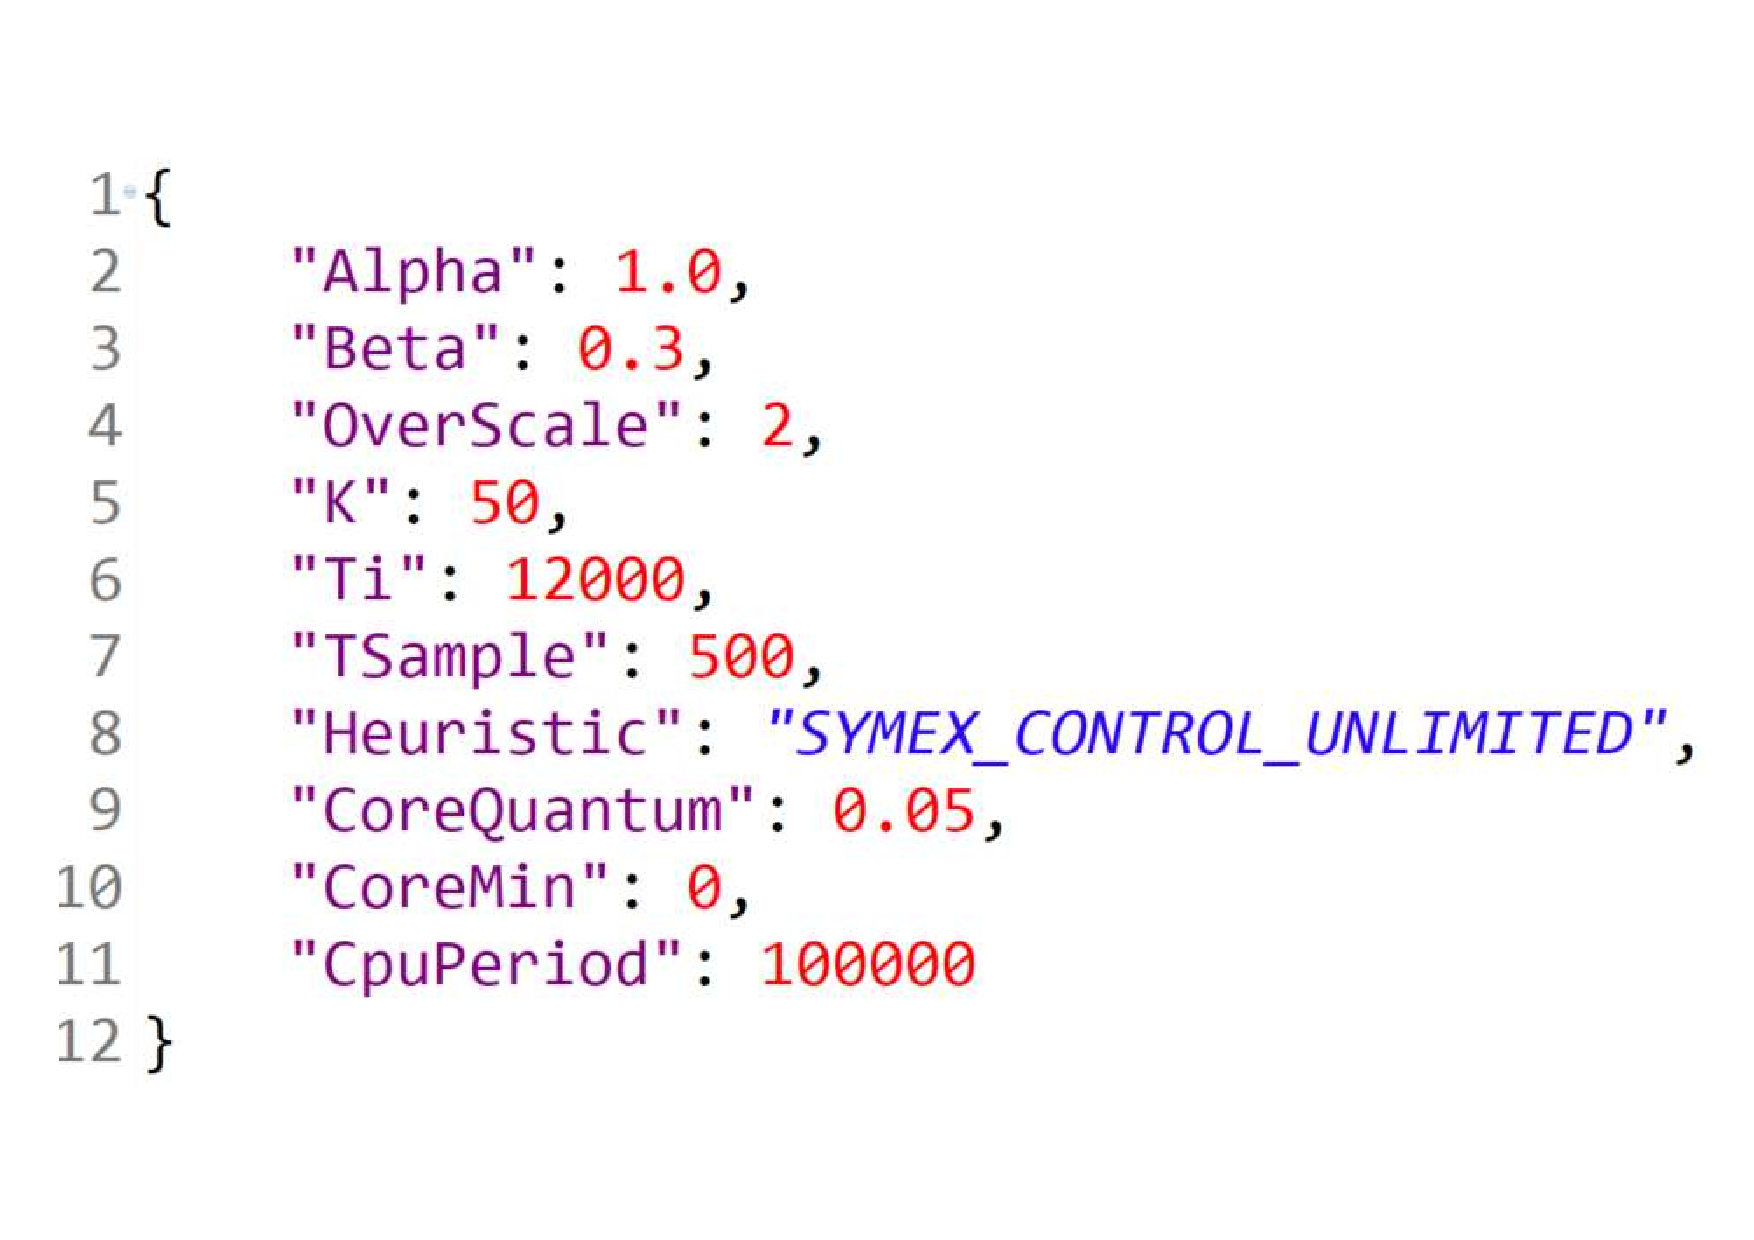
\includegraphics[width=\columnwidth]{images/xspark_symex_control_unlimited_parms.pdf}
	\caption{control.json \tool configuration parameters.}
	\label{fig:xSparkDagSymbConfigParms}
\end{figure}
\begin{figure}[thbp]
	\centering
	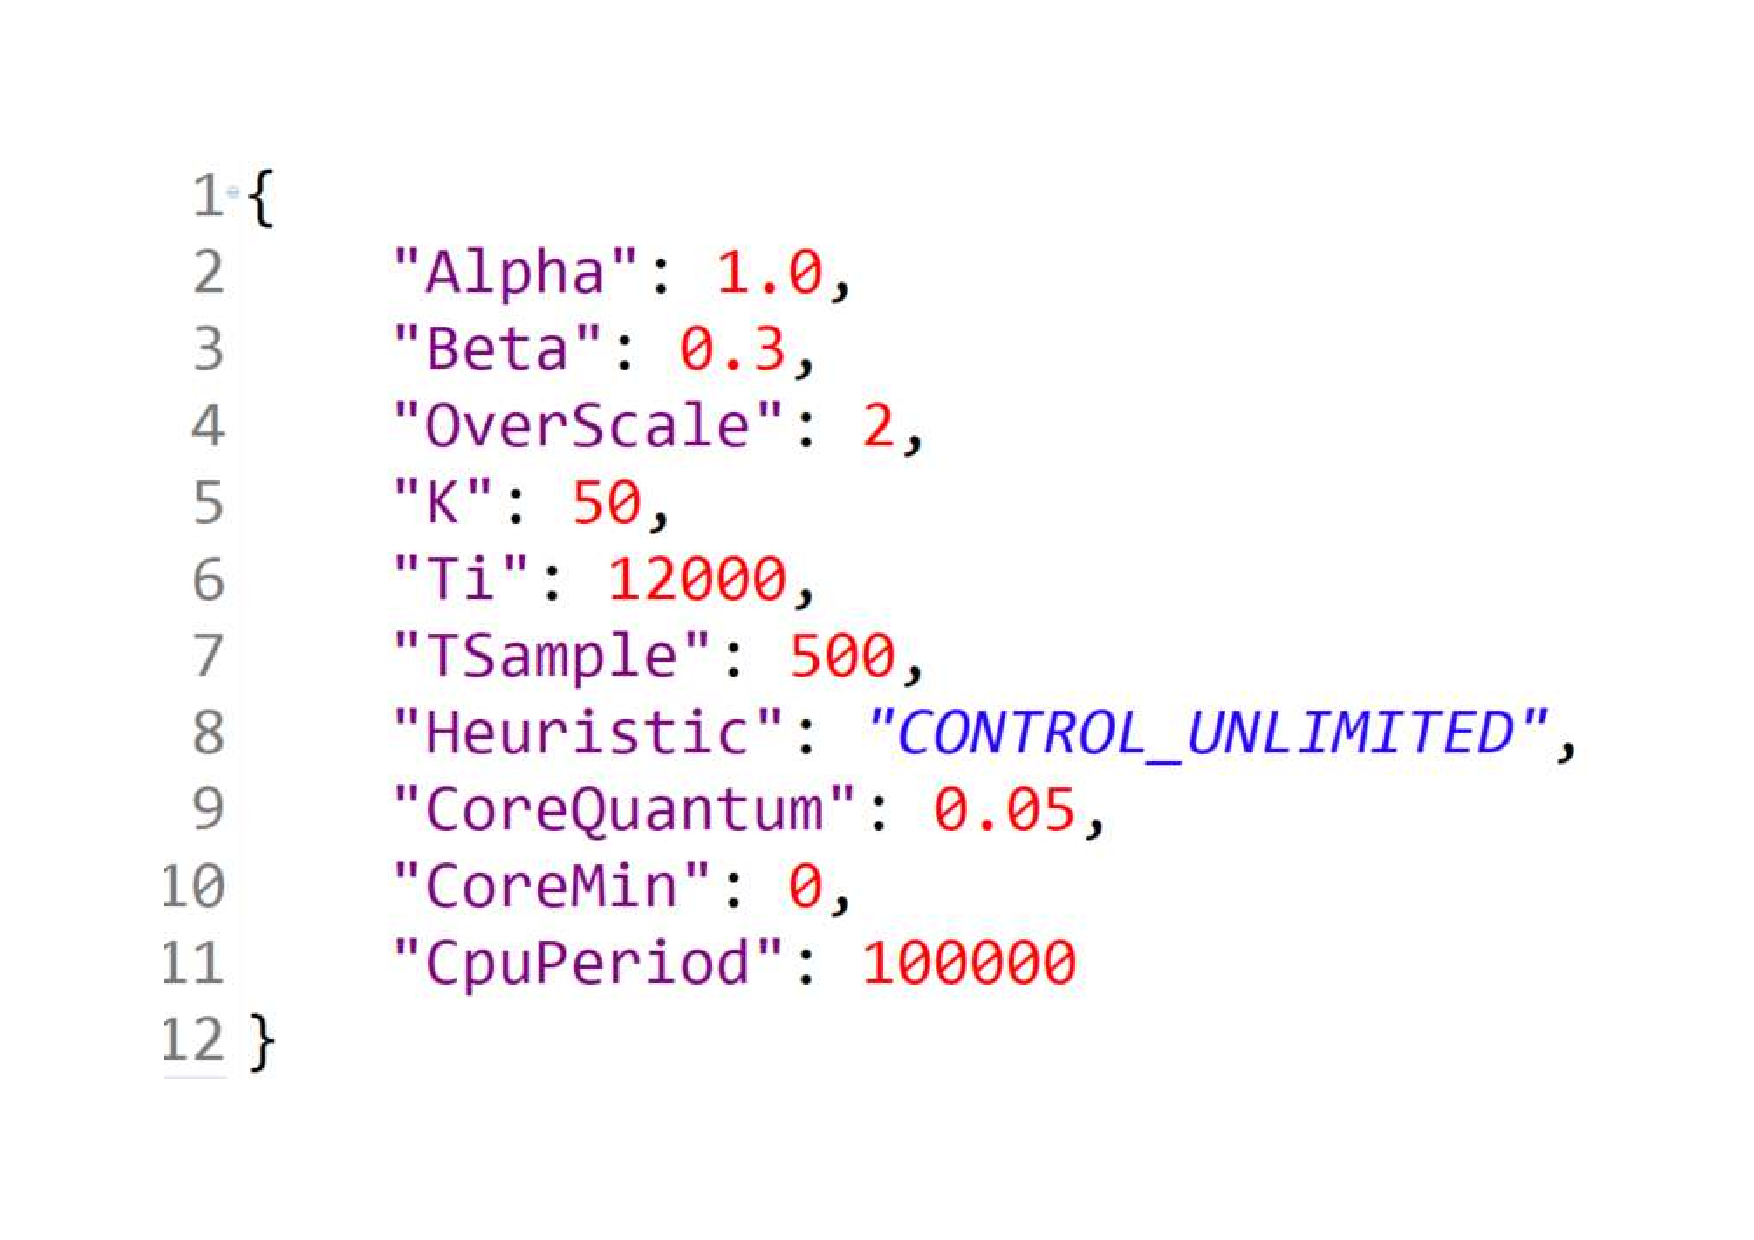
\includegraphics[width=\columnwidth]{images/xspark_control_unlimited_parms.pdf}
	\caption{control.json \cSpark configuration parameters.}
	\label{fig:xSparkConfigParms}
\end{figure}

\section{Tested Applications}\label{sec:tested_apps}
We performed the experiments with two applications: 
PromoCalls and Louvain. PromoCalls is an example application that was developed at Politecnico di Milano in the Deib Labs\footnote{\url{https://github.com/seepep/promocalls}}.
It resembles a batch application from a telecommunications company that calculates promotional discounts based on the number of daily domestic and foreign calls (calls longer than a parametric threshold) made by customers. 
If a customer makes more than  $min_l$ local long calls or more than $min_a$ abroad long calls (or both) in a day, she may receive discounts on the calls made in that day, in the last $m$ months, or in the current month. 
Only some or all of the discounts may be applied to the customer depending on the possible combinations of the trigger conditions. 
PromoCalls uses Spark to efficiently analyze the data of all calls and calculate the applicable discounts.
PromoCalls was used as a reference application during the development of SEEPEP and for a preliminary assessment of the accuracy of the technique used.

Instead, to evaluate our approach to a real world application, we selected Louvain, a Spark implementation of the Louvain algorithm~\cite{Louvain} that we downloaded from a highly ranked GitHub repository\footnote{\url{https://github.com/Sotera/spark-distributed-louvain-modularity}}. Louvain uses \textit{GraphX}, a Spark library specialized for graph processing, suitable for representing large user networks and analyzing communities belonging to these networks.

\section{Experiments}\label{sec:experiments}
The experiments were performed on each of the applications subjected to the tests following the procedure described below, which consists of three distinct phases:
\begin{enumerate}[$1 $]
	\item Execution of \dSymb to obtain the path conditions and generate the launchers corresponding to each identified path.
	\item Profiling the application subject to the test with the launchers generated and obtaining the plans for each path.
	\item Use of tool to control the execution of the application by feeding it with input data sets larger by one order of magnitude compared to those used to generate the launchers.
\end{enumerate}
We have generated at least one large data set for each profiled path. We also set a reasonable deadline, that is $ 20\% $ longer than the minimum deadline, measured by running the application on Spark configured to use all the resources available on the clusters, and with the same data sets used in the experiments .

The datasets were randomly generated using \dSymb.

The comparison of \tool with the original \cSpark version has been done, for each application under test, identifying the best and worst cases, i.e. the paths with the lowest and highest number of stages\footnote{In case two paths have the same number of stages, we chose the path with the shortest/longest execution time  respectively for the best/worst case.}. In this way, we have quantified the error that \cSpark can generate due to the fact that it ignores which plan was used in the profiling phase.

\subsection{Results}
Results produced by\tool for PromoCalls and Louvain tools, up to the profiling phase, are shown in Tables~\ref{Table:Check:Promo} and ~\ref{Table:Check;Louvain}. Column $Path$ lists the paths found by \dSymb: $8$ unique paths were discovered in both cases. 

Column $Found?$ shows whether or not \dSymb succeeded in generating a test case (and thus a corresponding profiling launcher) for the identified paths: it was successful in generating test cases for all path of PromoCalls, instead it was able to identify 6 out of 8 possible paths of Louvain\footnote{The two paths of Louvain for which \dSymb was not successful in identifying a corresponding test case were manually inspected. In any case, the proof that either these paths are infeasible, or an input datasets can be identified that exercise these paths, is missing.}. As a matter of fact, we currently have no clue if Louvain can execute these program paths or not.)

Column $Jobs$ and column $Stages$ report  the number of jobs and stages collected when profiling the launchers with \cSpark, which range between 3 and 9 jobs, 3 and 9 stages for Promocalls, and 11 and 17 jobs, 73 and 364 stages for Louvain, respectively. These data are not available for the two paths of Louvain for which \dSymb did not generate a launcher.
In both tables, we marked with $^\bullet$ and $^\dagger$ the paths that correspond to the best and worst case, respectively, of each application. 

\begin{table}[thbp]
	\centering
	\hspace{1cm}
	\parbox{.48\linewidth}{
		%\hspace{0.1cm}
		\begin{tabular}{c|c|c|c}
			\toprule
			\multicolumn{1}{c|}{\textbf{Path}} &  \multicolumn{1}{c|}{\textbf{Found?}}   & \multicolumn{1}{c|}{\boldmath$\#Jobs$}  &  \multicolumn{1}{c}{\boldmath$\#Stages$}    \\
			%\rotatebox{90}{\textbf{Path}} &  
			%\rotatebox{90}{\textbf{Found?}}   & 
			%\rotatebox{90}{\boldmath$\#Jobs$}  &  %\rotatebox{90}{\boldmath$\#Stages$}    \\
			\midrule
			$0$ & Yes  & 6 & 6  \\	
			$1^{\bullet}$ & Yes  &  3 &  3 \\	
			$2$ & Yes & 7  & 7 \\
			$3$ & Yes &  6 & 6 \\
			$4$ & Yes & 8  & 8  \\
			$5$ & Yes & 7 & 7 \\
			$6^{\dagger}$ & Yes & 9 & 9 \\
			$7$ & Yes &  8 & 8 \\
			\bottomrule
		\end{tabular}
		\caption{\boldmath$PromoCalls$ paths.}
		\label{Table:Check:Promo}
	}
%\end{table}
%\begin{table}[thbp]
	\centering
	\parbox{.48\linewidth}{
		%	\vspace{0.78cm}
		\vspace{2cm}
		\hspace{0.5cm}
		\begin{tabular}{c|c|c|c|c}
			\toprule
			\multicolumn{1}{c|}{\textbf{Path}} &  \multicolumn{1}{c|}{\textbf{Found?}}   & \multicolumn{1}{c|}{\boldmath$\#Jobs$}  &  \multicolumn{1}{c}{\boldmath$\#Stages$}    \\
			%\rotatebox{90}{\textbf{Path}} &  
			%\rotatebox{90}{\textbf{Found?}}   & 
			%\rotatebox{90}{\boldmath$\#Jobs$}  &  %\rotatebox{90}{\boldmath$\#Stages$}    \\
			\midrule
			$0$ & Yes  &  11 & 149 \\	
			$1$ & Yes & 17 & 364  \\	
			$2^{\dagger}$ & Yes & 17 & 364 \\
			$3$ & Yes & 11  & 149  \\
			$4$ & No & - & - \\
			$5$ & No & -  & - \\	
			$6$ & Yes & 17 & 364 \\
			$7^{\bullet}$ & Yes & 8  & 73  \\		
			\bottomrule
		\end{tabular}
		\caption{\boldmath$Louvain$ paths.}
		\label{Table:Check;Louvain}
	}
	
\end{table}
\begin{table}[tbhp]
	\centering
	\begin{tabular}{r|c|c|c|c|c|c}
		%\toprule
		\multicolumn{1}{c|}{\textbf{Experiment}}   &
		%\multicolumn{1}{R{90}{1em}{|}}{\textbf{Experiment}} & \multicolumn{1}{c|}{\boldmath$deadline\,[s]$}  &  \multicolumn{1}{c|}{\boldmath$exec\_time\,[s]$}  & \multicolumn{1}{c|}{\boldmath$Violation$} &  \multicolumn{1}{c|}{\boldmath$error$}    & \multicolumn{1}{c|}{\boldmath$core\_alloc\,[\frac{core}{s}]$}  & \multicolumn{1}{c|}{\boldmath$penalty$}   \\
		%\rotatebox{90}{\textbf{Experiment}}   &
		\rotatebox{90}{\boldmath$deadline\,[s]$}  &  \rotatebox{90}{\boldmath$exec\_time\,[s]$}  & \rotatebox{90}{\boldmath$violation$} &  \rotatebox{90}{\boldmath$error$}    & \rotatebox{90}{\boldmath$core\_alloc\,[\frac{core}{s}]$}  & \rotatebox{90}{\boldmath$penalty$}   \\
		\midrule
		$xSpark_s$  & $91.4$   & $90.3$   & $No$   & $1.2\%$   & $41.3$   & $-$  \\
		$P_0 \,\,xSpark_w$  & $91.4$   & $88.0$   & $No$   & $3.8\%$   & $53.0$   & $28.3\%$  \\
		$xSpark_b$  & $91.4$   & $143.0$   & $Yes$   & $56.4\%$   & $30.6$   & $\infty$  \\
		\midrule
		$xSpark_s$  & $56.4$   & $46.0$   & $No$   & $18.4\%$   & $56.2$   & $-$  \\
		$P_1 \,\,xSpark_w$  & $56.4$   & $45.3$   & $No$   & $19.6\%$   & $56.5$   & $0.5\%$  \\
		$xSpark_b$  & $56.4$   & $55.3$   & $No$   & $1.9\%$   & $38.2$   & $\text{-}33.6\%$  \\
		\midrule
		$xSpark_s$  & $107.8$   & $106.3$   & $No$   & $1.3\%$   & $39.2$   & $-$  \\
		$P_2 \,\,xSpark_w$  & $107.8$   & $104.0$   & $N$   & $3.5\%$   & $52.1$   & $32.9\%$  \\
		$xSpark_b$  & $107.8$   & $175.0$   & $Yes$   & $62.4\%$   & $29.0$   & $\infty$  \\
		\midrule
		$xSpark_s$  & $87.5$   & $86.0$   & $No$   & $1.7\%$   & $42.4$   & $-$  \\
		$P_3 \,\,xSpark_w$  & $87.5$   & $83.0$   & $No$   & $5.1\%$   & $53.5$   & $26.2\%$  \\
		$xSpark_b$  & $87.5$   & $138.0$   & $Yes$   & $57.8\%$   & $30.1$   & $\infty$  \\
		\midrule
		$xSpark_s$  & $147.6$   & $146.0$   & $No$   & $1.1\%$   & $37.0$   & $-$  \\
		$P_4 \,\,xSpark_w$  & $147.6$   & $130.0$   & $No$   & $11.9\%$   & $51.4$   & $38.9\%$  \\
		$xSpark_b$  & $147.6$   & $228.0$   & $Yes$   & $54.5\%$   & $28.4$   & $\infty$  \\
		\midrule
		$xSpark_s$  & $77.0$   & $75.3$   & $No$   & $2.2\%$   & $41.0$   & $-$  \\
		$P_5 \,\,xSpark_w$  & $77.0$   & $70.0$   & $No$   & $9.1\%$   & $53.7$   & $30.9\%$  \\
		$xSpark_b$  & $77.0$   & $122.0$   & $Yes$   & $58.4\%$   & $29.7$   & $\infty$  \\
		\midrule
		$xSpark_s$  & $122.2$   & $120.3$   & $No$   & $1.5\%$   & $39.2$   & $-$  \\
		$P_6 \,\,xSpark_w$  & $122.2$   & $120.7$   & $No$   & $1.2\%$   & $43.6$   & $11.3\%$  \\
		$xSpark_b$  & $122.2$   & $204.0$   & $Yes$   & $67.0\%$   & $27.9$   & $\infty$  \\
		\midrule
		$xSpark_s$  & $112.1$   & $110.7$   & $No$   & $1.3\%$   & $39.2$   & $-$  \\
		$P_7 \,\,xSpark_w$  & $112.1$   & $100.0$   & $No$   & $10.8\%$   & $53.0$   & $35.2\%$  \\
		$xSpark_b$  & $112.1$   & $180.0$   & $Yes$   & $60.6\%$   & $28.8$   & $\infty$  \\
		
		\bottomrule
	\end{tabular}
	\caption{Results for \boldmath$PromoCalls$}
	\label{Table:PerfPromo}
\end{table}


\begin{table}[htbp]
	\centering
	\begin{tabular}{r|c|c|c|c|c|c}
		%\toprule
		\multicolumn{1}{c|}{\textbf{Experiment}}   &
		%\multicolumn{1}{R{90}{1em}{|}}{\textbf{Experiment}} & \multicolumn{1}{c|}{\boldmath$deadline\,[s]$}  &  \multicolumn{1}{c|}{\boldmath$exec\_time\,[s]$}  & \multicolumn{1}{c|}{\boldmath$Violation$} &  \multicolumn{1}{c|}{\boldmath$error$}    & \multicolumn{1}{c|}{\boldmath$core\_alloc\,[\frac{core}{s}]$}  & \multicolumn{1}{c|}{\boldmath$penalty$}   \\
		%\rotatebox{90}{\textbf{Experiment}}   &
		\rotatebox{90}{\boldmath$deadline\,[s]$}  &  \rotatebox{90}{\boldmath$exec\_time\,[s]$}  & \rotatebox{90}{\boldmath$violation$} &  \rotatebox{90}{\boldmath$error$}    & \rotatebox{90}{\boldmath$core\_alloc\,[\frac{core}{s}]$}  & \rotatebox{90}{\boldmath$penalty$}   \\
		\midrule
		$xSpark_s$  & $184.3$   & $180.1$   & $No$   & $2.3\%$   & $35.9$   & $-$  \\
		$P_0 \,\,xSpark_w$  & $184.3$   & $142.0$   & $No$   & $23.0\%$   & $46.1$   & $28.4\%$  \\
		$xSpark_b$  & $184.3$   & $222.3$   & $Yes$   & $20.6\%$   & $15.2$   & $\infty$  \\
		\midrule
		$xSpark_s$  & $228.0$   & $227.0$   & $No$   & $0.4\%$   & $32.3$   & $-$  \\
		$P_1 \,\,xSpark_w$  & $228.0$   & $222.0$   & $No$   & $2.6\%$   & $33.2$   & $2.8\%$  \\
		$xSpark_b$  & $228.0$   & $329.3$   & $Yes$   & $44.4\%$   & $7.4$   & $\infty$  \\
		\midrule
		$xSpark_s$  & $292.8$   & $290.7$   & $No$   & $0.7\%$   & $32.3$   & $-$  \\
		$P_2 \,\,xSpark_w$  & $292.8$   & $289.0$   & $No$   & $1.3\%$   & $32.5$   & $0.5\%$  \\
		$xSpark_b$  & $292.8$   & $429.0$   & $Yes$   & $46.5\%$   & $7.0$   & $\infty$  \\
		\midrule
		$xSpark_s$  & $228.7$   & $226.0$   & $No$   & $1.2\%$   & $35.5$   & $-$  \\
		$P_3 \,\,xSpark_w$  & $228.7$   & $211.3$   & $No$   & $7.6\%$   & $41.4$   & $16.6\%$  \\
		$xSpark_b$  & $228.7$   & $292.0$   & $Yes$   & $27.7\%$   & $16.0$   & $\infty$  \\
		\midrule
		$xSpark_s$  & $163.0$   & $159.4$   & $No$   & $2.2\%$   & $38.4$   & $-$  \\
		$P_6 \,\,xSpark_w$  & $163.0$   & $158.0$   & $No$   & $3.0\%$   & $39.8$   & $3.8\%$  \\
		$xSpark_b$  & $163.0$   & $242.0$   & $Yes$   & $48.5\%$   & $8.5$   & $\infty$  \\
		\midrule
		$xSpark_s$  & $156.0$   & $139.0$   & $No$   & $10.9\%$   & $33.2$   & $-$  \\
		$P_7 \,\,xSpark_w$  & $156.0$   & $131.5$   & $No$   & $15.7\%$   & $43.6$   & $31.4\%$  \\
		$xSpark_b$  & $156.0$   & $152.7$   & $No$   & $2.1\%$   & $30.9$   & $-7.0\%$  \\
		\bottomrule
	\end{tabular}
	\caption{Results for $Louvain$}
	\label{Table:Louvain}
	\vspace{-8mm}
\end{table}

The effectiveness of \tool to control the execution of the tested applications, whose inputs were fed with large datasets, is measured by the results of our experiments that are summarized in Tables~\ref{Table:PerfPromo} and ~\ref{Table:Louvain}. These tables also include the results obtained with the original version of \cSpark, tuned on the worst and best case datasets mentioned above, and allow us to compare \tool against \cSpark. The meaning of each column of the tables is explained here below.

For each profiled path $P_i$, column $Experiment$ indicates the data obtained with \tool ($xSpark_s$), and \cSpark configured with the worst-case dataset ($xSpark_w$) and with the best-case dataset ($xSpark_b$), respectively. 
In column $deadline$ we show the set deadline in seconds. 
In column $exec\_time$ the actual execution time of the application is reported in seconds, as the average of $5$ iterations of the experiments (for a total of $120$ executions of PromoCalls (8 paths $\times$ 5 repetitions $\times$ 3 modes) and $90$ executions of Louvain). 
In column $violation$ we show the deadline violations (i.e., $exec_time > deadline$). 
The error  is quantified in column $error$, defined as:
%
\[
error = \frac{|deadline - exec\_time|}{deadline}\cdot100\%
\]
%
that is, the percentage change vs. the deadline of the distance between the actual execution time and the deadline itself. In general the smaller $error$, the more efficient is the resource allocation, provided that the deadline is not violated, since less resources were used to meet the goal. On the other hand, if the deadline is violated, to smaller errors correspond shorter delays. Note that if the deadline were to be considered strict, the penalty for a violation would be considered of infinite value~\cite{shin1994real}.
In column $core\_alloc$ we show the average core allocation during the execution, that is defined as:
%
\[
core\_alloc = \frac{\sum_{s = 0}^{exec\_time} coresAllocatedAtSecond(s)}{exec\_time} 
\]
%

We remark that the maximum value of $core\_alloc$ is $64$ core/second since $64$ is the number of cores provided by the cluster used for these experiments.

In the last column $penalty$ we quantify the performance of \tool compared to  \cSpark when executing the same experiment: $penalty$ is defined as:
\[
penalty = 
\begin{cases}
\frac{ru_{WORST|BEST}-ru_{SEEPEP}}{ru_{SEEPEP}}\cdot 100\%,& \text{if } violation = No \\
\infty,              & \text{if } violation = Yes
\end{cases}
\]

Remarkably in our experiments, \tool never violated the deadline, hence $penalty$ measures the amount of resources that either $xSpark_w$ or $xSpark_b$ have used with respect to \tool. E.g. a $penalty$ of 30\% means that \cSpark used 30\% more resources than \tool. Instead, a negative $penalty$ means that \cSpark used less  resources than \tool. Lastly, when the deadline is violated by either $xSpark_w$ or $xSpark_b$, we consider $penalty$ to be infinite~\cite{shin1994real}. 

As evidenced by the data in Tables~\ref{Table:PerfPromo} and ~\ref{Table:Louvain},  $xSpark_b$ violated the deadline in $7$ out of $8$ paths in the experiments with PromoCalls, and 5 out of 6 paths in the experiments with Louvain. This is due to the optimistic, yet wrong, estimations made in the profiling phase. To explain this behaviour, we have to consider that, for Promocalls, $xSpark_b$ computes the local deadlines and the resource allocation  as if the \plan always consisted of $3$ stages. As a consequence, in all the experiments but $P_1$ (which is the actual best-case path) \cSpark under allocates resources, resulting in the execution time eventually exceeding the deadline by as much as $51.9\%$. We measured the highest error displacement, equals to $67.0\%$, with the worst-case path $P_6$ where \cSpark faces the widest gap between the profiling estimations and the actual runtime workload. 

In the same tables we can appreciate that $xSpark_w$ does not violate any deadline, on the contrary it causes the earlier termination of the applications in most of the cases, with an $error$ between 1.2\% and 19.6\% in the case of PromoCalls, and between 1.3\% and 23\% in the case of Louvain. This beahoiur depends on the pessimistic, yet wrong, estimations made in the profiling phase,  that mistakenly consider the worst-case path of the applications to represent all the possible paths.
When considering paths $P_1$, $P_4$, $P_5$ and $P_7$ of PromoCalls,  and  $P_0$, $P_3$ and $P_7$ of Louvain, the error is greater than $7\%$, leading  to significantly sub-optimal resource allocations. 

Remarkably, and on the contrary, \tool does not violate any deadline and successfully provides an efficient resource allocation. The average error measured in our experiments is equal to $3.6\%$ for PromoCalls, where for $xSpark_b$ and $xSpark_w$ is $52.4\%$ and $8.1\%$, respectively, and equal to $2.9\%$ for Louvain, where $xSpark_b$ and $xSpark_w$ have an average error of $31.6\%$ and $8.9\%$, respectively.

The data in columns $core\_alloc$ confirm that \tool outperforms the performance of $xSpark_b$ and $xSpark_w$. $xSpark_b$ underestimates allocated resources so as to make \cSpark violate the deadlines in all experiments, except for path $P_1$ in PromoCalls and path $P_7$ in Louvain (the best cases). In the latter two cases, profiled data match the runtime workload, leading $xSpark_b$ to outperform both $xSpark_w$ and \tool, and minimizes the error and used resources. 

\tool allocates an average of $25.5\%$ fewer resources in PromoCalls, and $13.9\%$ in Louvain, with respect to $xSpark_w$.

From the results of our experiments we can evince a positive answer to both research questions $RQ_1$ and $RQ_2$, because \tool effectively and efficiently controls the allocation of resources during the execution of PromoCalls and Louvain, keeping the execution times within considered deadlines with significantly smaller errors and consuming a lower amount of resources than the original version of \cSpark.

\section{Threats to Validity}
\label{sec:ThreatsToValidity}

We came up with a considerable trial effort, which has led us to perform a total of $226$ experiments on two different applications: a paradigmatic example and a real-world application taken from GitHub. We have shown that \dSymb was able to find a test-case for 14 out 16 of the application paths statically identified with symbolic execution, and demostrated how \cSpark could take advantage from the integration with \dSymb. In this section, we highlight the threats that may constrain the validity of our current results~\cite{wohlin2006empirical}:

\textbf{Internal Threats}.  The test cases generated by \dSymb have been slightly modified to increase the size of the datasets (without breaking the path conditions) for the execution of the experiments. This was done to ensure that we could test the desired paths and reliably obtain different repetitions of the experiments. However, data sets were not created in a totally random way. For this reason, we have preliminary executed some experiments with completely randomly created data sets and have obtained a similar result to the one presented.
A broader set of experiments could be done to address this aspect as a matter for future developments.

\textbf{External Threats}. A limit to the generality of the experiments and of the solutions tested may derive from the assumption underlying the choice of the Spark applications that we have considered. We have chosen two applications: one that uses Spark's core transformations and one that uses the \textit{GraphX} entry for graph analysis. To increase the degree of generality of evaluations, an extension of the number and variety of Spark applications is desirable, taking into consideration different types, such as those that exploit machine learning solutions and use SQL.

%Profiling as it is currently done constitutes an additional limitation of the approach used. In fact, a profiling session is required for each test case (launcher) found by \dSymb, but this could become a problem when the number of program paths becomes too high. A desirable direction for a future work could be the improvement of this part of the tool chain. The improvement could be achieved through the adoption of a branch-based criterion to select profiling executions, replacing the current path-based criterion. The underpinning rationale is that since the execution of all the program branches assures that any possible \plan of the program has been profiled at least once; then, after profiling, we can map the profiled \plans on the paths (and then the path conditions) that include the corresponding program branches. This optimization might also mitigate the issues with paths that our test generator fails to exercize, such as the 2 uncovered paths that we experienced in Louvain.

%\textbf{Concept and Conclusion Threats}. 
The experiments demonstrate the validity of our idea, namely that the knowledge of the different \plans generated by the Spark applications helps to analyze and control their performance and execution time. Furthermore, we show that an approach based simply on knowledge of the worst case may be sufficient to limit the number of deadline violations, but is significantly less efficient than the one we obtain with our solution. The results obtained are statistically robust and they show only a small variance. 
